\documentclass[12pt]{article}


\usepackage[dvips,letterpaper,margin=0.75in,bottom=0.5in]{geometry}
\usepackage{cite}
\usepackage{slashed}
\usepackage{graphicx}
\usepackage{amsmath}

\begin{document}
\newcommand{\pt}           {\ensuremath{ p_{\rm T} }}
\newcommand{\Et}           {\ensuremath{ E_{\rm t}     }}

\let\divsymb=\div % rename builtin command \div to \divsymb
\newcommand{\gv}[1]{\ensuremath{\mbox{\boldmath$ #1 $}}} 
\newcommand{\grad}[1]{\gv{\nabla} #1} % for gradient
\renewcommand{\div}[1]{\gv{\nabla} \cdot #1} % for divergence


%\let\vaccent=\v % rename builtin command \v{} to \vaccent{}
%\renewcommand{\v}[1]{\ensuremath{\mathbf{#1}}} % for vectors
%\let\divsymb=\div % rename builtin command \div to \divsymb
%\newcommand{\uv}[1]{\ensuremath{\mathbf{\hat{#1}}}} % for unit vector
\newcommand{\abs}[1]{\left| #1 \right|} % for absolute value
\newcommand{\avg}[1]{\left< #1 \right>} % for average




\let\underdot=\d % rename builtin command \d{} to \underdot{}
\renewcommand{\d}[2]{\frac{d #1}{d #2}} % for derivatives
\newcommand{\dd}[2]{\frac{d^2 #1}{d #2^2}} % for double derivatives
\newcommand{\pd}[2]{\frac{\partial #1}{\partial #2}} % for partial derivatives
\newcommand{\pdd}[2]{\frac{\partial^2 #1}{\partial #2^2}} % for double partial derivatives
\newcommand{\pdc}[3]{\left( \frac{\partial #1}{\partial #2} \right)_{#3}} % for thermodynamic partial derivatives

\newcommand{\planewave}{e^{\textstyle i\vec{k} \cdot \vec{x}}}
\newcommand{\radialwave}{\frac{1}{r} \, e^{\textstyle ikr}} 

\title{Interference and Diffraction}
\author{Michael Mulhearn}

\maketitle

\section{Introduction}

The linearity of the wave equation leads to the Superposition
Principle, which states that the sum of two solutions to the wave
equation is also a solution to the wave equation.  The wave that
results from adding two waves according to the superposition principle
can be larger or smaller than the original waves, due to constructive
or destructive interference.  When an incident wave interacts with an
obstacle or a slit of approximately the same dimension as the
wavelength of the wave, the interference of the resulting waves is
referred to as diffraction.  We'll examine these processes
quantitatively in this lecture.

\section{The Wave Equation in Three Dimensions}

The Wave Equation we derived for one dimension extends to three dimensions by simply adding analogous terms corresponding to $y$ and $x$:
\begin{equation}
\frac{1}{v^2} \cdot \pdd{u(x,y,z,t)}{t} = \pdd{u(x,y,z,t)}{x} + \pdd{u(x,y,z,t)}{y} + \pdd{u(x,y,z,t)}{z} 
\end{equation}  
This form is a bit clumsy to write, so we write it this way:
\begin{equation}\label{eqn:wave3d}
\frac{1}{v^2} \cdot \pdd{u(x,y,z,t)}{t} = \left( \pdd{}{x} + \pdd{}{y} + \pdd{}{z} \right) u(x,y,z,t) 
\end{equation}  
And as physicists are generally lazy, the quantity in parenthesis is often even written $\grad^2$.

The equation 
\begin{equation}
u(x,y,z,t) = A \sin(kx - \omega t),
\end{equation}  
is a solution to the wave equation, because the partial derivatives with respect to $y$ and $z$ are both zero, and the left hand side was already shown to be a solution to the 1-D wave equation in variable $x$.  This solution is called a plane wave traveling in the $x$ direction.  The points where the wave reaches the maximum value form planes perpendicular to the $x$ axis, as shown in Fig.~\ref{fig:planewave}.  This is simply the 3-D extension of the waves we might see advancing toward a long straight  beach on a windy day, as in Fig.~\ref{fig:beachwave}.  We'll show in the homework that plane waves can head in any direction (not just $x$).

Another solution to the 3-D wave equation is a spherical wave:
\begin{equation}
u(r,t) = A \frac{1}{r} \sin(kr - \omega t),
\end{equation}
where $r$ is the usual radius of spherical coordinates:  $r = \sqrt{x^2+y^2+z^2}$.  Its not an easy calculation, but it can be shown that this is a solution to the 3-D wave equation.   You could probably grind through this calculation and carefully keep track of the bazillions of derivatives that are needed, but most people prefer to wait for more mathematical machinery which makes the calculation significantly easier.

The spherical wave is the equation for a wave which ripples outward from the origin in all directions, so that the peaks form spheres that ripple outward through the medium.  We can at least explain the factor of $1/r$ in front.  In the previous homework, we saw that the energy density of a wave was proportional to the amplitude of the wave {\em squared}.  As each wave front ripples outward it forms a sphere with surface area $4 \pi r^2$.  To conserve energy, therefore, the amplitude of the wave must fall as $1/r$, so that the surface area times amplitude squared is a constant, conserving energy.  You have seen this effect in 2-dimensions, as the diminishing size of ripples moving outward from a stone dropped into still water.

\begin{figure}[thb]
\begin{center}
{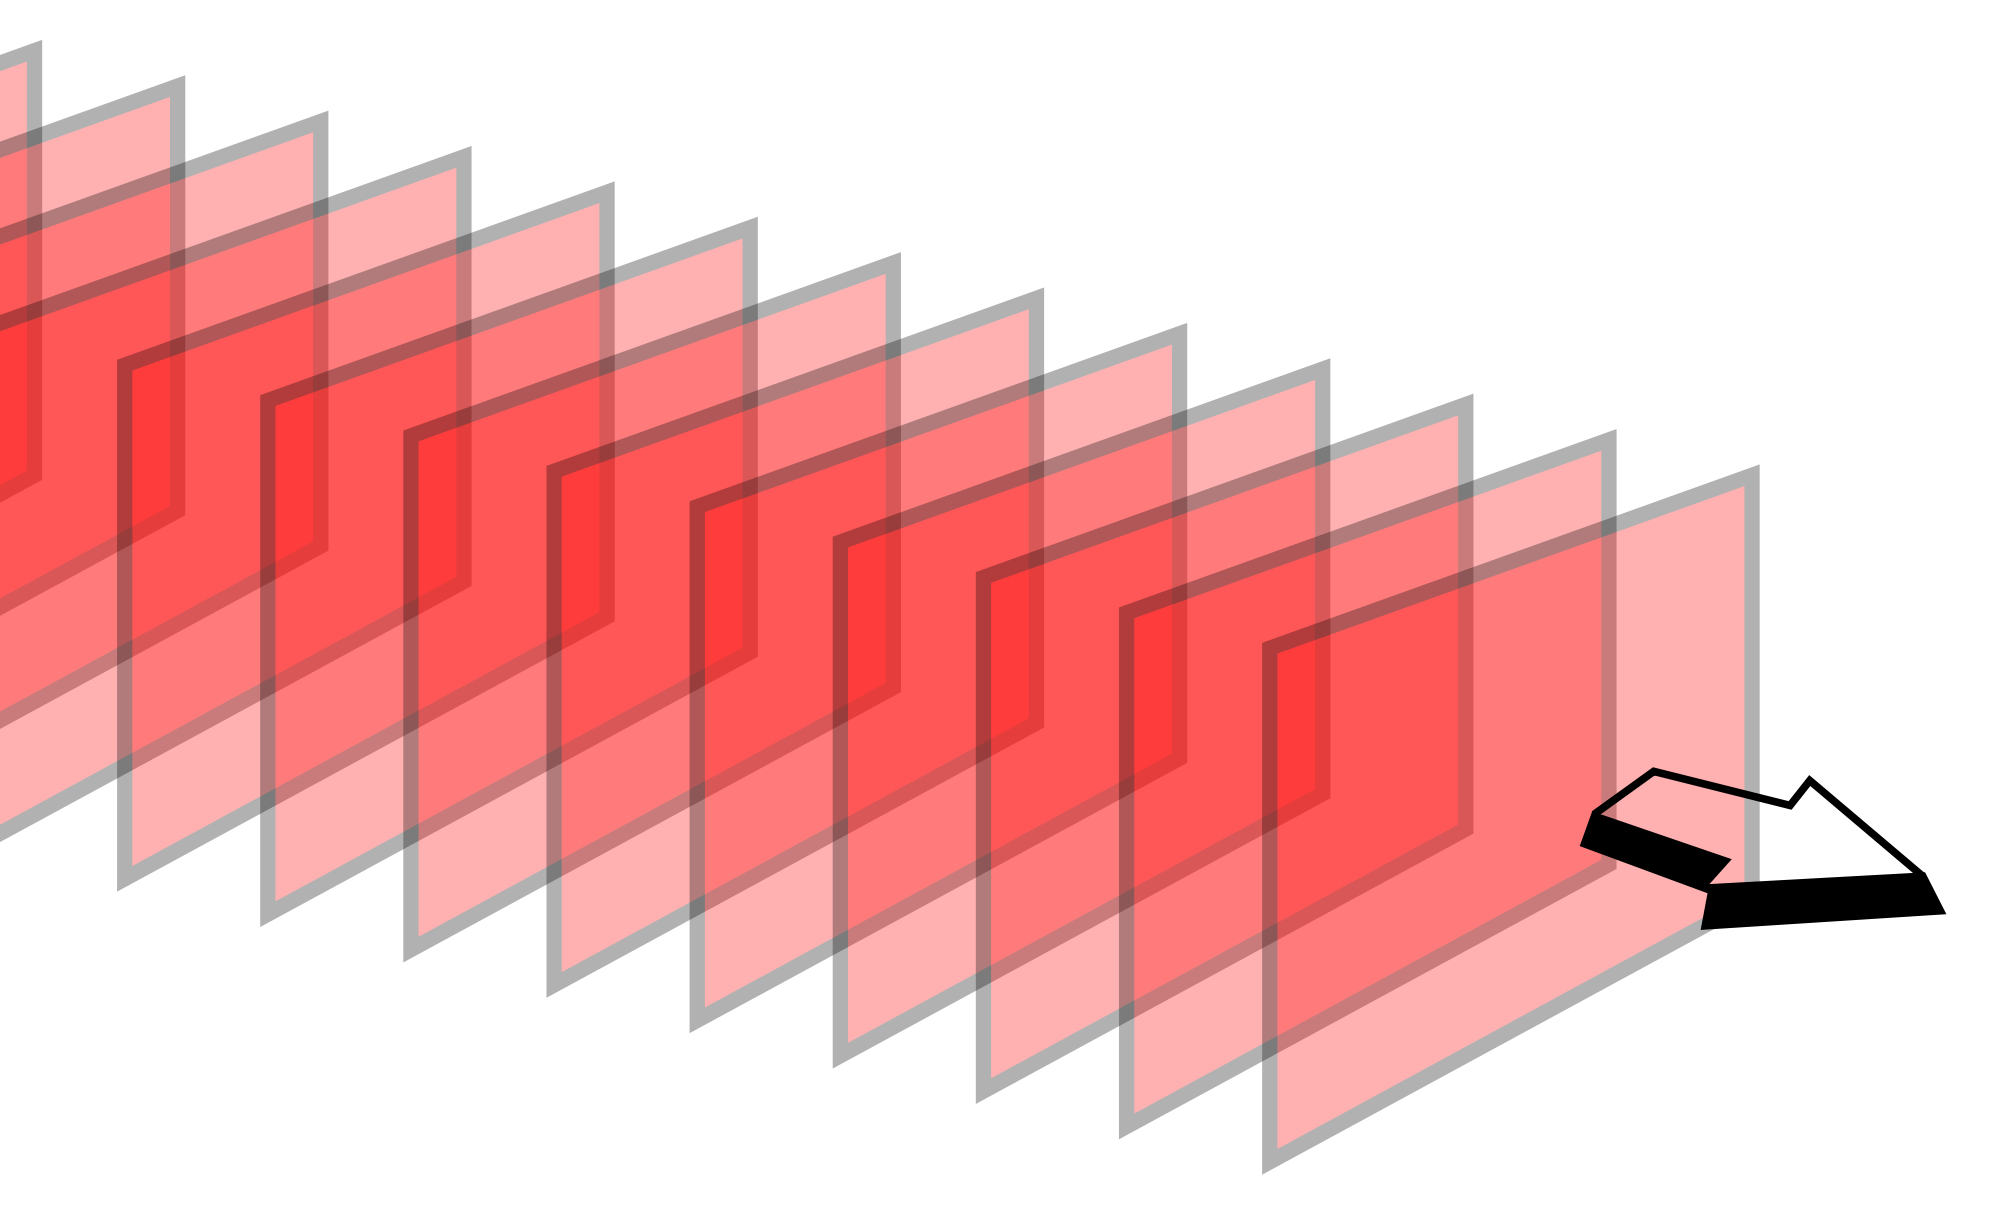
\includegraphics[width=0.55\textwidth]{figs/planewave.png}}
\end{center}
\caption{\label{fig:planewave}A plane wave.  The planes show the points where the wave reaches its maximum value, and these planes advance in the direction perpendicular to the plane at the wave speed in the medium. }
\end{figure}

\begin{figure}[thb]
\begin{center}
{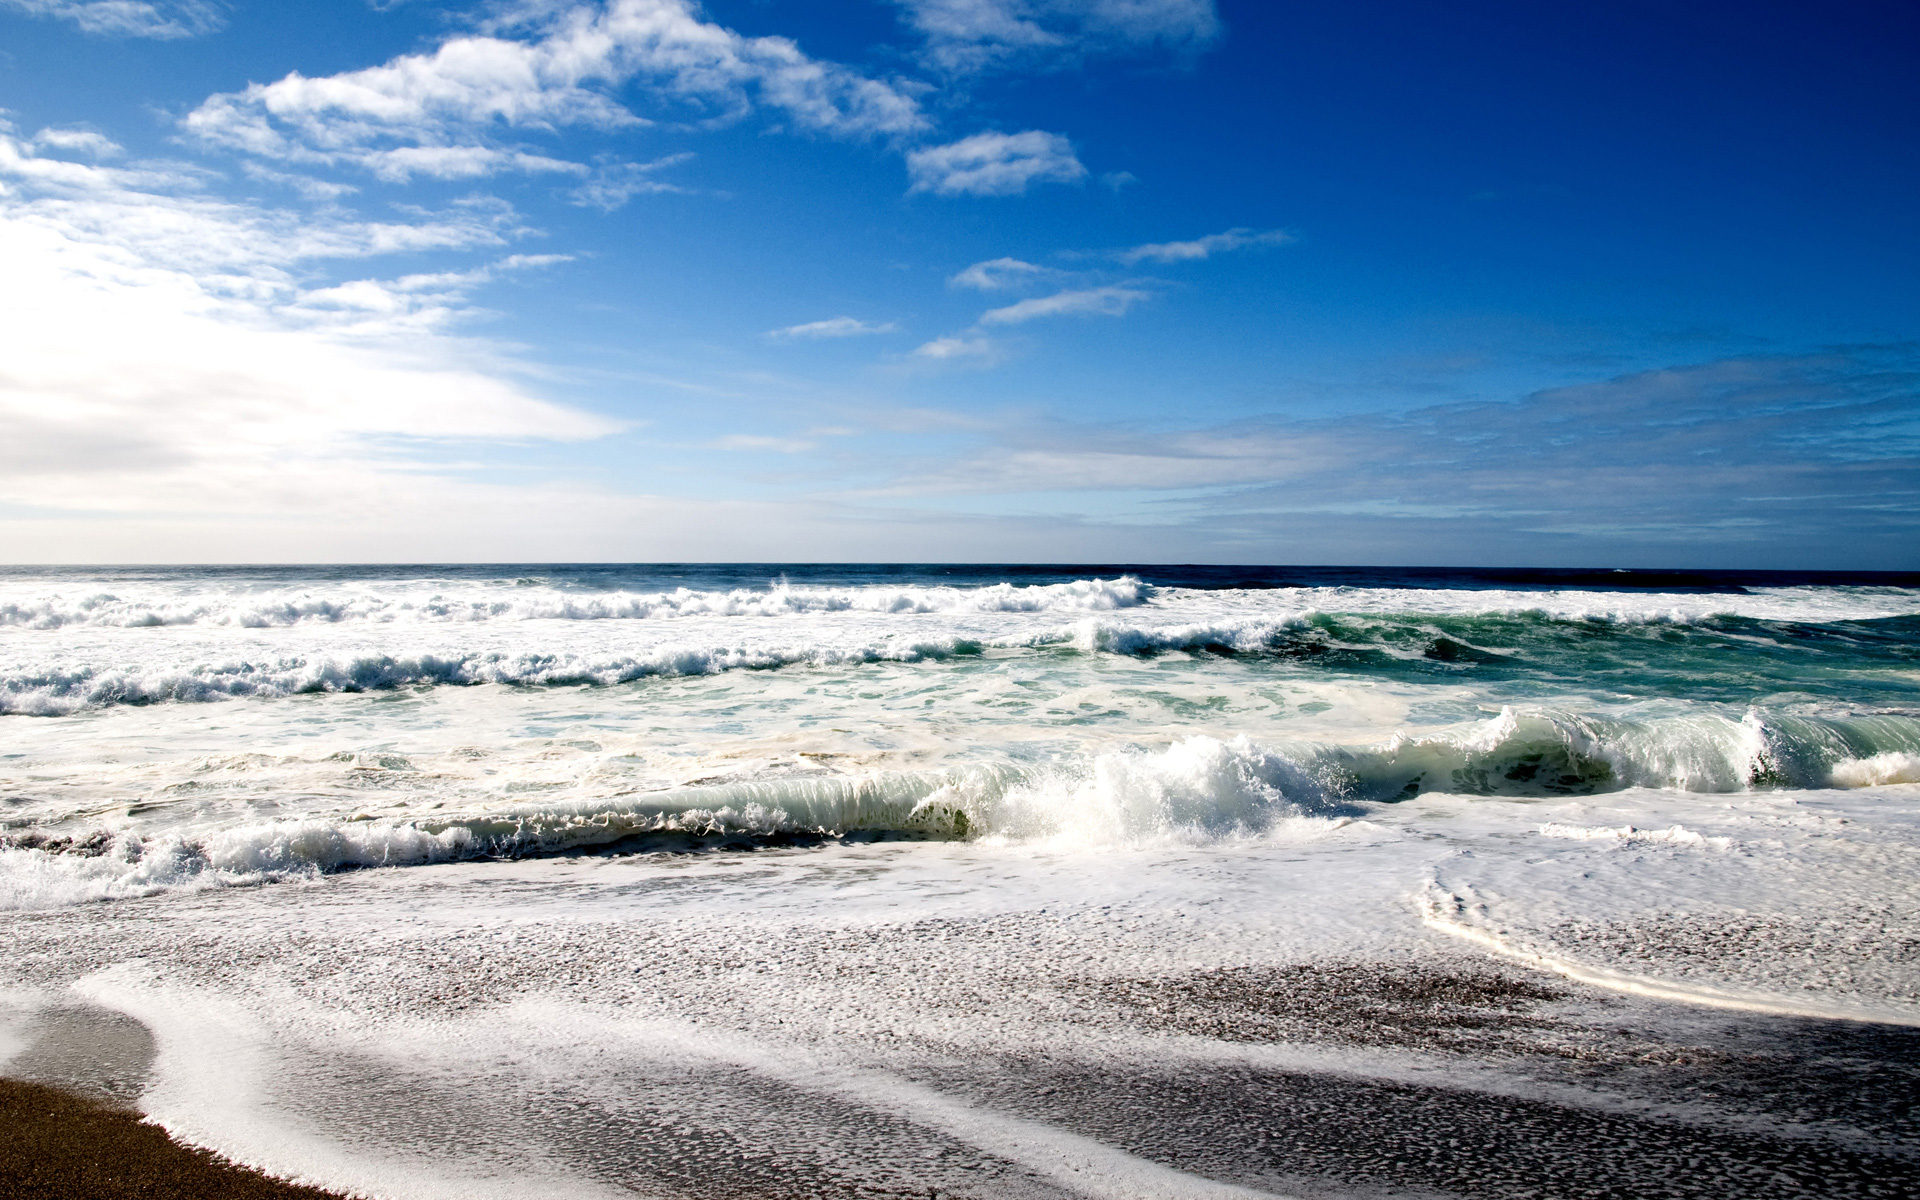
\includegraphics[width=0.55\textwidth]{figs/beach.jpg}}
\end{center}
\caption{\label{fig:beachwave} An example of a 2-D plane wave (approximately).}
\end{figure}

\begin{figure}[thb]
\begin{center}
{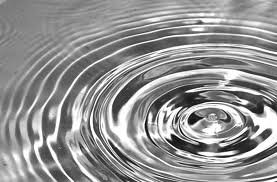
\includegraphics[width=0.55\textwidth]{figs/ripples.jpg}}
\end{center}
\caption{\label{fig:ripples} As water ripples move outward from a disturbance, they must decrease in size in order to conserve energy.}
\end{figure}


\section{Interference of Two Spherical Waves}

\begin{figure}[thb]
\begin{center}
{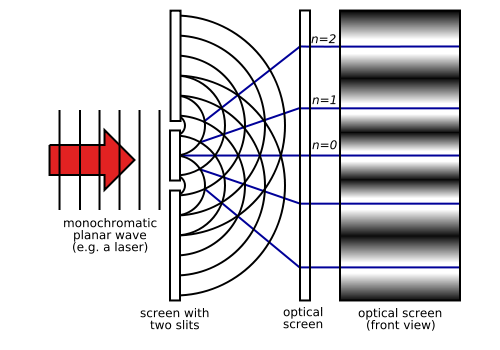
\includegraphics[width=0.55\textwidth]{figs/interference.png}}
\end{center}
\caption{\label{fig:interference} Interference of two circular waves}
\end{figure}

Suppose we shine a plane wave (such as from a laser) onto a screen into which two slits have been etched (this is the situation shown in Fig.~\ref{fig:interference}).  For now, we'll assume the slits have a width which is much smaller than the wavelength of the light, so they are effectively point sources of light on the other side of the screen.  The light from each of these point sources will spread out as a spherical wave.  We can calculate the resulting interference pattern:  the intensity of the observed light on a screen located far away from the slit.

\begin{figure}[thb]
\begin{center}
{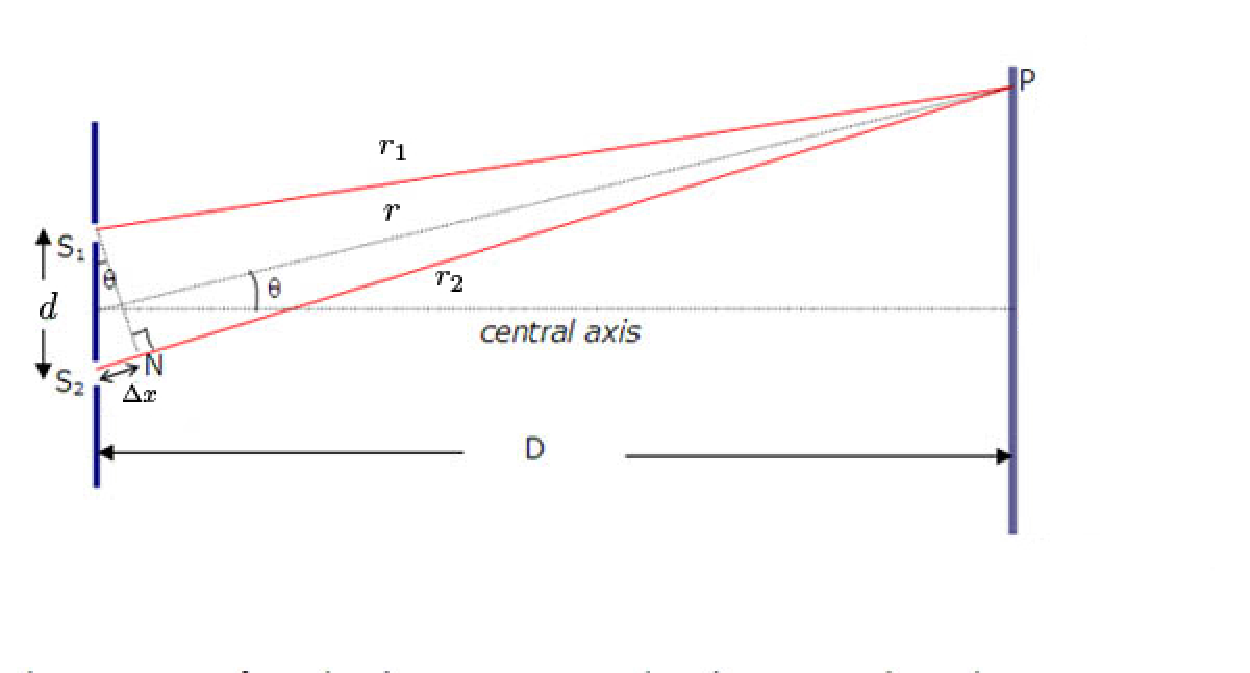
\includegraphics[width=0.85\textwidth]{figs/two-slit-geometry.pdf}}
\end{center}
\caption{\label{fig:geo} Geometry}
\end{figure}

The geometry for the situation is shown in Fig.~\ref{fig:geo}.  The slits are located a distance $d$ apart.  We showed in class that if the point $P$ is very far from the diffracting surface, the three lines labeled $r_1$, $r$, and $r_2$ are very nearly parallel, and the two angles labelled $\theta$ are approximately the same

  As a result, the difference in the lengths $r1$ and $r2$ is given by:
\begin{displaymath}
\Delta x = d \sin \theta
\end{displaymath}
We can therefore write
\begin{eqnarray*}
r_1 &=& r - \frac{d}{2} \sin \theta \\ \\
r_2 &=& r + \frac{d}{2} \sin \theta \\
\end{eqnarray*}

The amplitude at point P of the spherical wave emitted from slit S1 will be:
\begin{displaymath}
u_1 = \frac{A}{r_1} \sin(k r_1- \omega t)
\end{displaymath}
and from slit S2:
\begin{displaymath}
u_2 = \frac{A}{r_2} \sin(k r_2- \omega t).
\end{displaymath}
The wave that results from the interference of these two circular waves will be:
\begin{eqnarray*}
u(r,\theta,t) &=& \frac{A}{r_1} \sin(k r_1- \omega t) + \frac{A}{r_2} \sin(k r_2- \omega t).
\end{eqnarray*}
In this case, the screen is very far from the diffraction pattern, so we can make the approximation that
\begin{displaymath}
\frac{1}{r} = \frac{1}{r_2} = \frac{1}{r_1},
\end{displaymath}
however, the $\sin$ function, being periodic, can (and does) change quite dramatically with relatively small change in the value of $r$.  So we calculate
\begin{eqnarray*}
u(r,\theta,t) &=& \frac{A}{r_1} \sin(k r_1- \omega t) + \frac{A}{r_2} \sin(k r_2- \omega t) \\
&=& \frac{A}{r} \left( \sin(k r_1- \omega t) + \sin(k r_2- \omega t) \right) \\
&=& \frac{A}{r} \left( \sin(k r- \omega t - \frac{kd}{2}\sin\theta) + \sin(k r- \omega t +  \frac{kd}{2}\sin\theta) \right) \\
\end{eqnarray*}
To simplify further, we note that
\begin{eqnarray*}
\sin(\alpha + \beta) + \sin(\alpha - \beta) &=&  2 \sin (\alpha) \cos (\beta)
\end{eqnarray*}
And so we finally obtain:
\begin{equation}
u(r,\theta,t) =  \frac{2A}{r} \sin(k r- \omega t) \cos \left( \frac{kd}{2}\sin\theta \right)  
\end{equation}
We are interested in the intensity of the pattern as a function of $\theta.$  Note that while the term $\sin(kr-\omega t)$ depends on $\theta$, as $r = D \cos \theta$, there will still always be a time $t$ during each period for which this sine function takes on the maximum value of $1$.  So the time average of this factor squared will be the same at every position in the interference pattern:  $1/2$.  The time averaged intensity will therefore be:
\begin{equation} \label{eqn:interference}
I(\theta) \sim \cos^2 \left( \frac{kd}{2}\sin\theta \right) = \cos^2\left( \frac{\pi d \sin \theta}{\lambda}\right)
\end{equation}
 The cosine function is maximal at integer values of $\pi$, so the condition for constructive interference is:

\begin{eqnarray*}
\frac{kd}{2} \sin \theta_{nc}  &=& n \pi \\
\frac{\pi d}{\lambda} \sin\theta_{nc}  &=& n \pi \\
\sin\theta_{nc} &=& n \frac{\lambda}{d} \\
\end{eqnarray*}
for all possible integers $n$, exactly as calculated in the Q2 of Moore.
 
\section{Diffraction from a Single Slit}

\begin{figure}[thb]
\begin{center}
{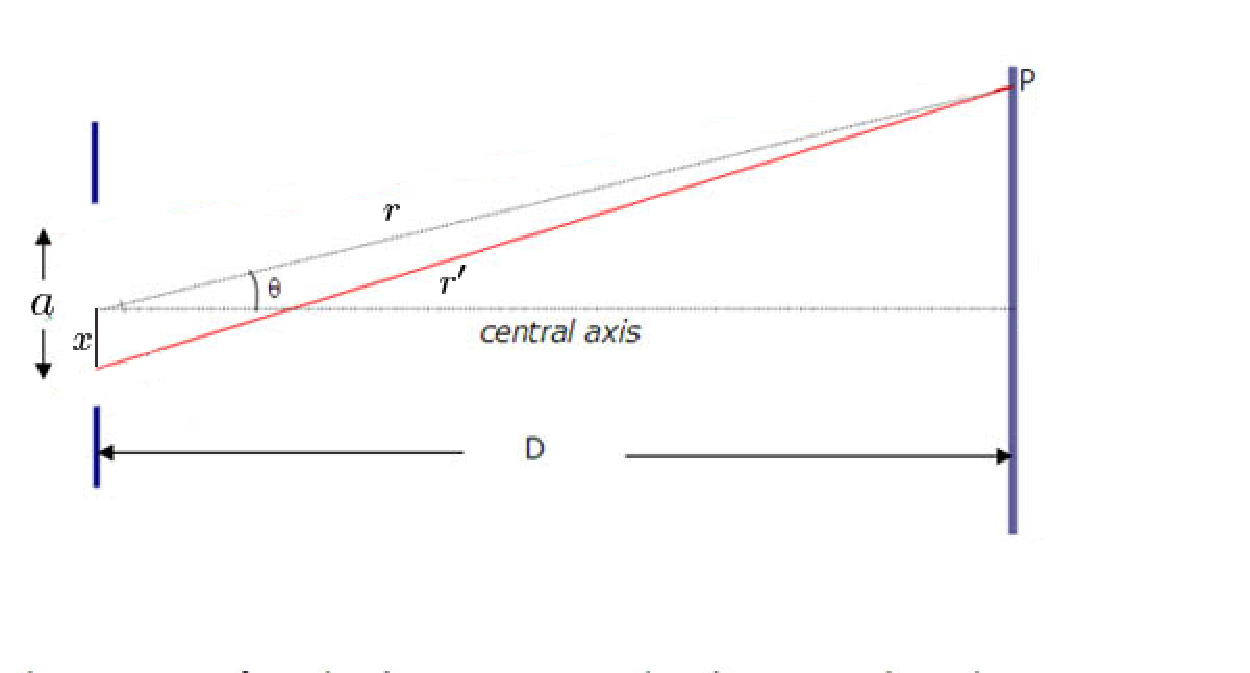
\includegraphics[width=0.85\textwidth]{figs/slitgeo.pdf}}
\end{center}
\caption{\label{fig:slitgeo} Geometry}
\end{figure}

Now we turn to the case of a plane wave of light incident on a screen in which a single slit of width $a$ has been etched, as shown in Fig.~\ref{fig:slitgeo}.  Huygen's principle allows us to calculate the wave on the right side of the screen by treating each point on the wavefront of the wave incoming from the left that {\em isn't stopped} by the screen, as a new point source of light resulting in a spherical wave heading toward the right.  For our slit, we will therefore be replacing the sum as calculated in the previous section for two spherical waves, with an integral across the slit parameterized by variable $x$.
\begin{displaymath}
\Sigma \; \to \; \frac{1}{a}\int_{-\frac{a}{2}}^{\frac{a}{2}}dx
\end{displaymath}
Each point $x$ along the slit will be a distance $r'(x)$ from the point $P$, with
\begin{displaymath}
r'(x) = r + x \sin \theta
\end{displaymath}
following the same geometric reasoning as for the two slit interference pattern.  The integral across all spherical waves along the slit, which will give us the total wave $u$, will be:
\begin{displaymath}
u = \frac{A}{a} \int_{-\frac{a}{2}}^{\frac{a}{2}}dx \frac{1}{r'(x)}\cos(kr'(x) - \omega t)
\end{displaymath}
Just as before we can make the approximation that
\begin{displaymath}
\frac{1}{r} = \frac{1}{r'(x)} 
\end{displaymath}
but not inside the rapidly oscillating sinusoidal wave.  We have:
\begin{eqnarray*}
u(r,\theta,t) &=& \frac{A}{ar} \int_{-\frac{a}{2}}^{\frac{a}{2}}dx \; \cos(kr - \omega t + kx \sin \theta ) \\
&=& \frac{A}{ar} \left( \frac{\sin(kr - \omega t - ka \sin \theta/2 )}{k \sin \theta/2} - 
\frac{\sin(kr - \omega t + ka \sin \theta/2 )}{k \sin \theta/2} \right) \\
&=& -\frac{A}{r} \, \sin(kr-\omega t) \cdot \frac{\sin(k a \sin \theta / 2)}{k a \sin \theta / 2}\\
\end{eqnarray*}
The last product is a ${\rm sinc}$ function:
\begin{displaymath}
{\rm sinc}(x) = \frac{\sin(x)}{x}
\end{displaymath}
Once again, the time average of $\sin^2(kr-\omega t)$ will give a value of $1/2$ so that the intensity will be:
\begin{equation}
I(\theta) \sim {\rm sinc}^2\left( \frac{k a \sin \theta}{2} \right) = {\rm sinc}^2\left( \frac{\pi a \sin \theta}{\lambda} \right)
\end{equation}
The resulting intensity and diffraction pattern are shown in Fig.~\ref{fig:diff-single}.
\begin{figure}[thb]
\begin{center}
{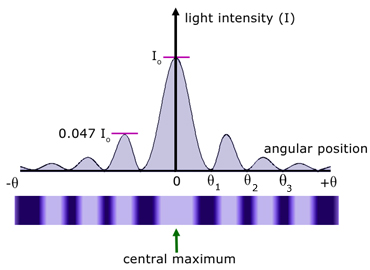
\includegraphics[width=0.65\textwidth]{figs/diff-single.jpg}}
\end{center}
\caption{\label{fig:diff-single} Intensity and observed diffraction pattern from a single slit.}
\end{figure}

\section{Diffraction from a Double Slit}

Next we consider diffraction from two slits each of width $a$ separated a distance $d$ away.  The diffraction pattern and interference patterns simply multiply, so that 
\begin{equation}
I(\theta) = I_0 \cdot \cos^2\left( \frac{\pi d \sin \theta}{\lambda}\right) 
\cdot {\rm sinc}^2\left( \frac{\pi a \sin \theta}{\lambda} \right)
\end{equation}
Example diffraction patterns from all the cases we calculated are shown in Fig.~\ref{fig:combined}

\begin{figure}[thb]
\begin{center}
{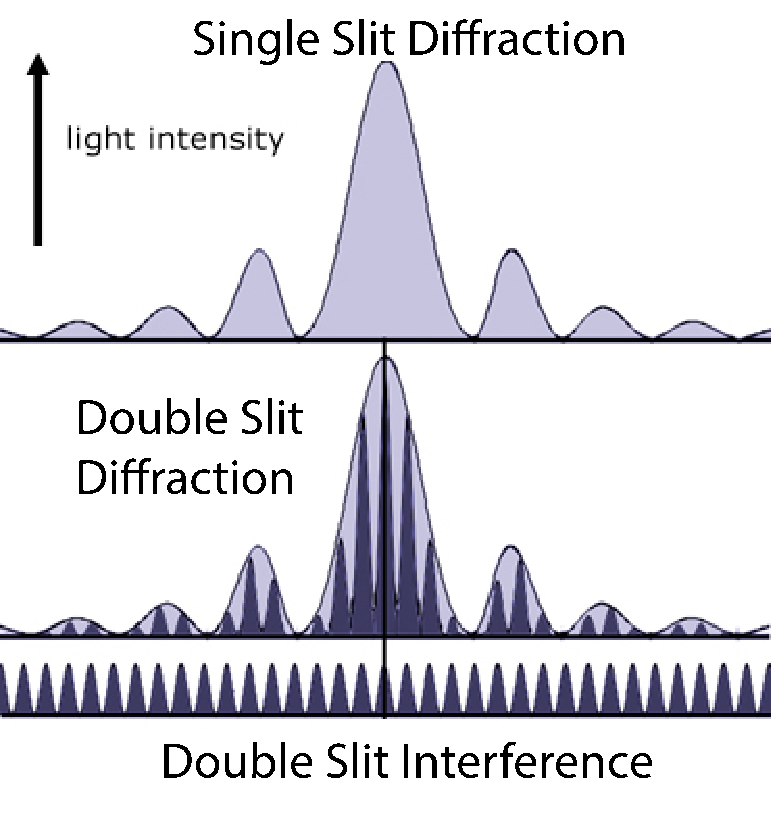
\includegraphics[width=0.45\textwidth]{figs/combined.pdf}}
\end{center}
\caption{\label{fig:combined} Diffraction and Interference patterns.}
\end{figure}

\newpage
\section{Homework Problems}

\noindent
{\em Problem 1:} Show that the function:
\begin{displaymath}
u(x,y,z,t) = A \cos(k_x \,x + k_y \, y + k_z \, z - \omega t)
\end{displaymath}
is a solution to the wave equation.  If we define $k^2 = k_x^2 + k_y^2 + k_z^2$ what is the relation between $\omega$, $k$, and the characteristic speed from the wave equation $v$?  This is the equation for a plane wave traveling in an arbitrary direction.

\vskip 0.5cm

\begin{figure}[thb]
\begin{center}
{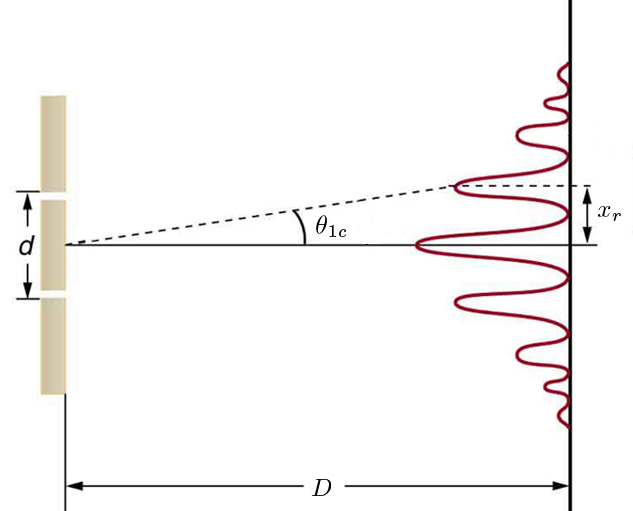
\includegraphics[width=0.45\textwidth]{figs/interference_exp.pdf}}
\end{center}
\caption{\label{fig:setup} Experimental Setup for Problems 2 and 3.}
\end{figure}

\noindent
{\em Problem 2:}   In class we produced an interference pattern much like that of Equation~\ref{eqn:interference} using green light $\lambda = 530~{\rm nm}$ and red light $\lambda = 650~{\rm nm}$.
We created an interference pattern on the board and measured the distance $x_{g}$ between the central peak and the next peak using green light.  We also measured the corresponding distance $x_{r}$ for red light.  (See Fig.~\ref{fig:setup}).  After class we also measured $sin(\theta_{1c}) = 0.35$ for green light.   What should we expect for the ratio of $x_r / x_g$?

\vskip 0.5cm

\noindent
{\em Problem 3:} There are a limited number of integer values of $n$ which produce a value for $\sin \theta_{nc}$ which has an absolute value less than one.  How many bright dots (i.e. possible values for $\theta_{nc}$) should we expect to find for the green laser?  How about for the red laser?


\vskip 0.5cm

\noindent
{\em Problems from Moore:} Q2: B2,5,8,9,14 S1,6,9,12 {R3}

\begin{itemize}

\item Hint on Q2.B2:  You are given both the width of the speakers and the distance between them so that you can calculate the distance $d$ from {\em center to center} of the speakers.

\item Hint on Q2.B9:  Assume that most of the sound is contained between the first destructive angle at $n=1$ and $n=-1$ (i.e. the first peak of the sinc function)

\item Hint on Q2.S9:  See Example Q2.4.  Also, just assume the wavelength of visible light is 550 nm.

\item Hint on Q2.S12:  5 Leagues is about 24 km.  Yellow hair will reflect visible light with $\lambda=575~{\rm nm}$.  You want to resolve a human head of about 20 cm.

\end{itemize}




\end{document}




